\documentclass[twocolumn]{el-author}

%\usepackage[...]{...}      This has been commented out as we are not using any additional packages here.  On the whole, they should be unnecessary.
\newcommand{\hH}{\hat{H}}
\newcommand{\D}{^\dagger}
\newcommand{\ua}{\uparrow}
\newcommand{\nc}{\newcommand}
\nc{\da}{\downarrow} \nc{\hc}{\hat{c}} \nc{\hS}{\hat{S}}
\nc{\bra}{\langle} \nc{\ket}{\rangle} \nc{\eq}{equation (\ref}
\nc{\h}{\hat} \nc{\hT}{\h{T}}\nc{\be}{\begin{eqnarray}}
\nc{\ee}{\end{eqnarray}}\nc{\rd}{\textrm{d}}\nc{\e}{eqnarray}\nc{\hR}{\hat{R}}\nc{\Tr}{\mathrm{Tr}}
\nc{\tS}{\tilde{S}}\nc{\tr}{\mathrm{tr}}\nc{\8}{\infty}\nc{\lgs}{\bra\ua,\phi|}\nc{\rgs}{|\ua,\phi\ket}
\nc{\hU}{\hat{U}}\nc{\lfs}{\bra\phi|}\nc{\rfs}{|\phi\ket}\nc{\hZ}{\hat{Z}}\nc{\hd}{\hat{d}}\nc{\mD}{\mathcal{D}}
\nc{\bd}{\bar{d}}\nc{\bc}{\bar{c}}\nc{\mc}{\mathcal}\nc{\ea}{eqnarray}\nc{\mG}{\mathcal{G}}\nc{\bce}{\begin{center}}
\nc{\ece}{\end{center}}
\date{20th February 2012}

\begin{document}

\title{Gram-Schmidt Transceiver for Non-Orthogonal Multicarriers}

\author{Daniel C. Ara\'ujo, A. Macilio P. Lucena, Jo\~ao C. M. Mota}


\abstract{In this letter, we design the Gram-Schmidt Non-Orthogonal Multicarrier (GS-NOMC) system to transmit information through an AWGN channel. We propose a new scheme of transmitter and receiver for $M$ non-orthogonal carriers and evaluate the system bit error rate by simulation for $M=2$. The simulated bit error rate (BER) of  GS-NOMC is compared with the Gram-Schmidt Frequency Division Multiplexing (GSFDM), which is a novel system proposed in the literature,  and with the Maximum Likelihood (ML) detector for non-orthogonal multicarriers. We show the performance results of GSFDM presented in recent article makes no sense and, in addition, the BER of the GS-NOMC system  is equal to  the optimum (ML). }

\maketitle

%\vspace{-5pt}
\section{Introduction}Non-orthogonal Frequency Division Multiplexing (NOFDM) systems are  a multicarrier modulation (MCM) scheme whose the orthogonality between the carriers are not maintained in order to increase the robustness of the system for doubly dispersive channels \cite{Kozek,Fang}. 

At work of Kozek \cite{Kozek}, NOFDM is designed using the Weyl-Heisenberg (W-H) functions system described by $g(t-kT)e^{j2\pi l\Delta ft}$, where $g(t)$ is the pulseshape, $1/T$ is the symbol rate, $\Delta f$ is the carrier separation and $l$=1, 2, ... . According to \cite{Kozek} the transmitted symbols in the NOFDM system can only be recovered if the carrier separation symbol rate ratio (csr) $\Delta fT\geq1$ avoiding the inter carrier interference (ICI). Otherwise, the information is lost.  

In \cite{Lucena}, a communication system that utilizes two non-orthogonal carriers with $\Delta fT < 1$, for AWGN channel, has been studied. It was first shown that, even for the condition of $\Delta fT<1$ the information is recovered and, for the ML detector, the system performance is identical to the orthogonal  case ($\Delta fT=1$ ), if $1\leq \Delta fT \leq 0.61$.

Recently, another work \cite{Fang} shows the possibility to recover the information under the condition $\Delta fT<1$. In \cite{Fang}, the proposed system is similar to \cite{Kozek}, the same idea of the W-H functions is applied to design the transmitted signal, but the csr condition of carrier separation is extended to the $\Delta fT<1$ at a cost to include several constraints on the pulseshape to decrease the ICI.

More recently, \cite{Zhang} presents the Gram-Schmidt Frequency Division Multiplexing (GSFDM) system whose the transceiver is based on Gram-Schmidt orthogonalization procedure. The authors claim the system performance for AWGN channel is equivalent to the BPSK system regardless of the number and the separation of carriers. 

At this letter, doing Gram-Schmidt procedure, we design the Gram-Schmidt Non-Orthogonal Multicarrier (GS-NOMC) system for $M$ non-orthogonal QPSK carriers with spectral overlapping
($\Delta fT<1$) and rectangular pulseshape. The system performance is equal to the one reported in \cite{Lucena} for $M=2$ and respect the Shannon's limit. On the other hand, the GSFDM has a spectral efficiency above Shannon's limit for some $\Delta fT$.
\vspace{-22,5pt}
\section{System Design}
Consider the equivalent baseband transmitted signal $s_k(t)$ of $M$ non-orthogonal carriers, shown in Figure 1, with spectral overlapping and  rectangular baseband pulse with unitary amplitude ($g(t)=1, 0\leq t<T$) described by the following equation:
\vspace{-5pt}
\begin{equation}\label{s(t)}
s_k(t)=\sum_{m=1}^{M}a_m[k]e^{j2\pi f_mt}, (k-1)T \leq t<kT, 
\end{equation}
$a_m[k]$  is QPSK symbol associated to carrier with central frequency $f_m$, $T$ is the symbol duration, $k \in \mathbb{N}$ and indicates the time interval. 

In order to project the GS-NOMC transmitter and receiver we perform the Gram-Schmidt procedure upon the signal defined by Eq. 1. Basically, we use a set of orthonormal functions from the linearly independent functions $e^{j2\pi f_1t}$ \ldots $e^{j2\pi f_Mt}$ \cite{Zhang} to decompose $s_k(t)$ into a orthonormal base of Gram-Schmidt.  Therefore, we can represent the signal $s_k(t)$ from Eq. \ref{s(t)} as following:

\begin{equation}\label{s(t)}
s_k(t)  =  \sum_{m=1}^{M}d_m[k]\phi_{m,k}(t), (k-1)T \leq t<kT, k \in \mathbb{N},
\end{equation}
\begin{eqnarray}
\phi_{m,k}(t)&=&\frac{\psi_{m,k}(t)}{\int\limits_{(k-1)T}^{kT}|\psi_{m,k}(t)|^2dt}, \nonumber \\
%\end{eqnarray}
\psi_{m,k}(t) &=& e^{j2\pi f_mt} -\sum_{i=1}^{m-1}\left(\int\limits_{(k-1)T}^{kT}e^{j2\pi f_mt}\phi^*_{i,k}(t)dt\right)\phi_{i,k}(t). \nonumber
\end{eqnarray}
The function $\phi_{m,k}(t)$ forms a orthogonal base and $d_m[k]=\int_{(k-1)T}^{kT}s(t)\phi ^*_{m,k}(t)dt$, $(k-1)T \leq t<kT$. It is the projection of the signal $s_k(t)$ over $\phi_{m,k}(t)$, where $m=1, \ldots, M$. As an example, consider $M=2$, thus:
\begin{equation} \label{fi1}
\phi_{1,k}(t) = \frac{e^{j2\pi f_1t}}{\sqrt{T}},  
\end{equation}
\begin{equation}\label{fi2}
\phi_{2,k}(t) = \frac{e^{j2\pi f_2t}-sinc(\Delta fT)e^{j2\pi \Delta fT(k-1/2)}e^{j2\pi f_1t}}{\sqrt{T(1-sinc^2(\Delta fT))}},  
\end{equation}
the equations for $d_1[k]$ and $d_2[k]$ can be written in the matrix form :

\begin{equation}\label{MatrixB}
\bold{d}[k]=\bold{B}[k]\bold{a}[k],
\end{equation}
where $\bold{d}[k]=[d_1[k] d_2[k]]^T$ and $\bold{a}[k]=[a_1[k] a_2[k]]^T$, and the projections $d_1[k]$ and $d_2[k]$ are:

\begin{equation} \label{d1}
d_1[k] =  a_1[k]\sqrt{T}+a_2[k]\sqrt{T}sinc(\Delta fT)e^{j2\pi \Delta fT(k-1/2) },
\end{equation}
\begin{equation}\label{d2}
d_2[k] =  a_2[k]\sqrt{T(1-sinc^2(\Delta fT))}, 
\end{equation}
and the matrix $\textbf{B}[k]$ is given by:
$$\scriptsize {
\textbf{B}(k)=\left(\begin{array}{cc} \sqrt{T}&\sqrt{T}sinc(\Delta fT)e^{j2\pi \Delta fT(k-1/2)}\\
0 & \sqrt{T(1-sinc^2(\Delta fT))}
\end{array}\right)}.\quad$$


\begin{figure}[!]
\begin{center}
\includegraphics[height=8cm]{GSFDM_Mcarrier-1.eps}%GSFDM_Mcarrier.eps GSFDMtwocarrier.eps
\caption{The GS-NOMC transmitter and receiver structure for $M$ non-orthogonal carriers in the channel AWGN.}
\label{GS-NOMC}
\end{center}
\end{figure}

The matrix $\bold{B}[k]$ performs a linear transformation on the QPSK symbols, which returns the projections in $\phi_{1,k}(t)$ and $\phi_{2,k}(t)$. Based on the Eq. \ref{MatrixB} and on the procedure described in \cite{Zhang}, we can generalize the linear system for $M$ carriers and design the GS-NOMC transmitter and receiver structure for $M$ carriers. All the system, including an AWGN channel, is illustrated at Figure \ref{GS-NOMC}. The input bit sequence is denoted by $\{b_k[n]\}$ and then it is mapped in $M$ complex sequence of QPSK symbols $a_1[k]$, $a_2[k]$, \ldots, $a_M[k]$. The signal $n_k(t)$, indicated in Figure \ref{GS-NOMC}, is a white Gaussian noise with zero mean and variance $N_0/2$. The received signal is $r_k(t)$, $r_1[k]$, $r_2[k]$, \ldots, $r_M[k]$ are the $M$ projections of $r_k(t)$ in the basis functions $\phi_{1,k}(t)$, $\phi_{2,k}(t)$, \ldots, $\phi_{M,k}(t)$ respectively at the discrete instant $k$. The Minimum Distance Detector estimates $d_1[k]$, $d_2[k]$, \ldots, $d_M[k]$ from $r_1[k]$, $r_2[k]$, \ldots, $r_M[k]$ respectively. After this, in Figure 1, the receiver performs a linear transformation on $\hat{d}_1[k]$, $\hat{d}_2[k]$, \ldots, $\hat{d}_M[k]$  to obtain estimated symbols $\hat{a}_1[k]$, $\hat{a}_2[k]$, \ldots $\hat{a}_M[k]$.
\vspace{-0.11in}
\section{Results and Discussion}
We simulate the system shown in Figure \ref{GS-NOMC} for $M=2$, $\Delta fT=1, 2/3$ and $1/3$. The results of the bit error rate (BER) are shown in Figure \ref{BER}.

Note that, the simulated system has the same performance with relation to the orthogonal case ($\Delta fT=1$) when we set $\Delta fT=2/3$. On the other hand, there is a loss of performance to $\Delta fT=1/3$. This results are differents from the ones presented by Zhang et al in \cite{Zhang}, where they show the GSFDM, in a AWGN channel, has the same performance (BER) of the BPSK modulation, regardless the $\Delta fT$ conditions. However, the BER of our designed system is equal to the ML detector performance reported by Lucena et al in \cite{Lucena}, where a similar two non-orthogonal system is proposed. It is interesting to observe that in \cite{Lucena} is shown there is no loss of performance if $1\geq \Delta fT \geq 0.61$.

It seems that the difference of BER among GS-NOMC and GSFDM is due to the QPSK symbols, which modulate directly the functions basis $\phi_{1,k}(t)$ and $\phi_{2,k}(t)$ in GSFDM system \cite{Zhang}. In this case, if we consider that $s_k(t)$ is independent from the factor $\sqrt{T}$ present in Eq. \ref{fi1}, \ref{fi2}, \ref{d1} and \ref{d2}, the linear transformation, defined by Eq. \ref{MatrixB} could be associated to the GSFDM, if $\bold{B}[k]=\sqrt{T}\bold{I}$,  $\bold{I}$ is the identity matrix. On the other hand, this condition is true if only if $\Delta fT=1$ (orthogonal case), which contradicts the results in \cite{Zhang}. 

\begin{figure}[H]
\begin{center}
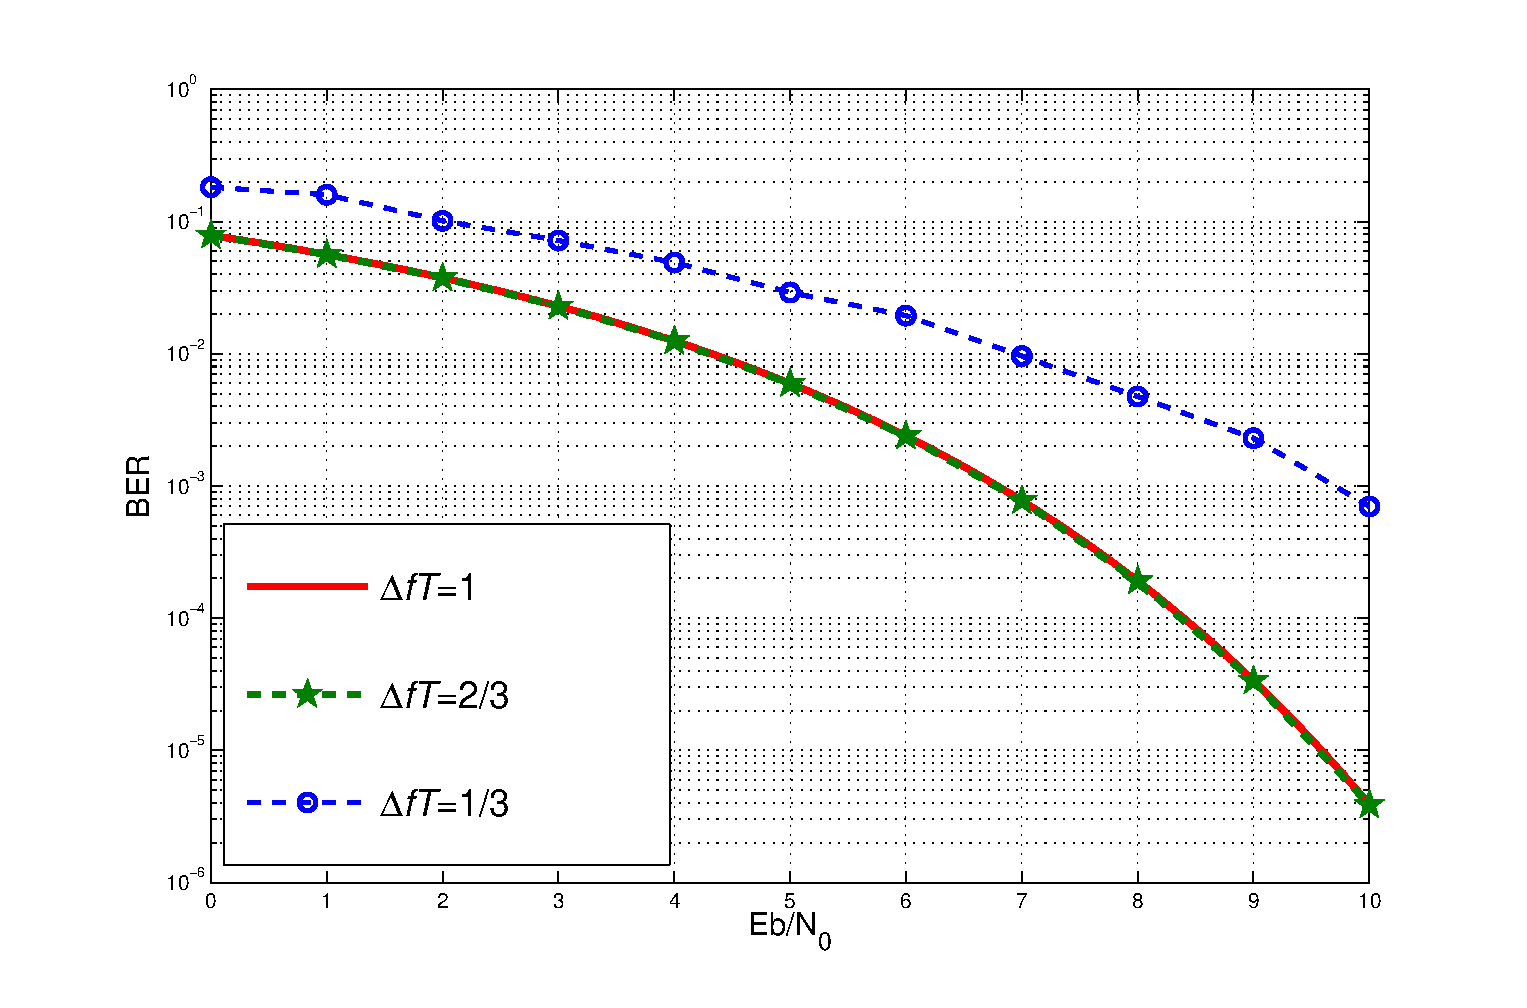
\includegraphics[height=6cm]{fig1_IET2.eps}
\caption{BER of GS-NOMC system for two carriers and $\Delta fT$=1, 2/3 and 1/3.}
\label{BER}
\end{center}
\end{figure}

The GS-NOMC performance suggests that there is a improvement on the spectral efficiency. Due to this, we calculate its efficiency, considering only the main lobe, as following:
\begin{eqnarray}
\eta=\frac{PM}{(M-1)\Delta fT + 2}, \nonumber
\end{eqnarray}
where $P$ is the number of bits in each carrier and $M$ is the number of carriers. The system represented in Figure \ref{GS-NOMC}, considering $\Delta fT=2/3$, $M=2$ and QPSK symbols, has a spectral efficiency $\eta=3/2$ bps/Hz, at the level of BER=$10^{-5}$, whereas to the orthogonal case ($\Delta fT=1$) has $\eta=4/3$ bps/Hz. Therefore, the GS-NOMC has an improvement with relation to the spectral efficiency, when compared to the orthognal case, as expected.

The GSFDM performance is the same one of the BPSK system independently of the number and the separation of carriers \cite{Zhang}, this suggest a great improvement on the spectral efficiency. However, if this is true we can make $M \to \infty$ and the spectral efficiency is $\eta=P/\Delta fT$. Considering $\Delta fT=1/4$ and QPSK symbols the spectral efficiency of GSFDM, at the level of BER=$10^{-5}$,  will be about 8 bps/Hz which is 2 bps/Hz above Shannon's limit \cite{Proakis}!
\vspace{-5pt}
\section{Conclusion}

GS-NOMC system for $M$ carries is designed and simulated for $M=2$. The BER results of the developed system show us a improvement at the spectral efficiency in relation to the two orthogonal carriers. The GS-NOMC performance is identical to the one presented in \cite{Lucena}. However, the BER of GSFDM system is better than the optimum detector shown in \cite{Lucena}. This result suggests a misunderstood in the implementation of GSFDM system by Zhang et al in \cite{Zhang}. We verify that such situation makes the spectral efficiency  of GSFDM system, like implemented in \cite{Zhang},  to be better than the Shannon's limit. 

We conclude that our system implement the optimum detector for non-orthgonal carriers, however, we know the increase of branches at the receiver in Figure \ref{GS-NOMC} will result in a increase of complexity of the system. Therefore, as a continuation of our research,  we will replace the Minimum Distance Detector block at the receiver for a linear or non-linear equalizer to retrieve the transmitted symbols. This will decrease the complexity of the receiver.

%\vskip3pt
%\ack{This work has been supported by The IET}

\vskip5pt
\noindent \textbf{Author's affiliation}:\\
\noindent Daniel Costa Ara\'ujo (Signal and Information Processing Group-SIPG, Federal University of Cear\'a-UFC, Brazil), daniel.c.araujo@gmail.com;\\
\noindent Ant\^onio Macilio Pereira Lucena (Northeast Regional Center of
National Institute of Space Research-INPE and Fortaleza University-UNIFOR, Brazil) macilio@roen.inpe.br;\\
\noindent Jo\~ao C\'esar Moura Mota (SIPG, Dept. of Teleinformatics Engineering, UFC, Brazil), mota@gtel.ufc.br.


%\vskip3pt

%\noindent E-mails: \\
%1. daniel.c.araujo@gmail.com; \\
%2. macilio@roen.inpe.br; \\
%3. mota@gtel.ufc.br .
%\vspace{-8pt}

\begin{thebibliography}{}

\bibitem{Kozek}
Kozek, W.; Molisch, A.F.;  "Nonorthogonal pulseshapes for multicarrier communications in doubly dispersive channels," Selected Areas in Communications, IEEE Journal on , vol.16, no.8, pp.1579-1589, Oct 1998.
\bibitem{Fang}
Fang-ming Han; Xian-da Zhang;  "Wireless multicarrier digital transmission via weyl-heisenberg frames over time-frequency dispersive channels," Communications, IEEE Transactions on , vol.57, no.6, pp.1721-1733, June 2009.
\bibitem{Zhang}
Peijian Zhang; Li Fang; Wei Jiang; Daoben Li; "A novel orthogonal transmission scheme for non-orthogonal multi-carrier signal," Broadband Network and Multimedia Technology (IC-BNMT), 2010 3rd IEEE International Conference on , vol., no., pp.467-471, 26-28 Oct. 2010
\bibitem{Lucena}
de Lucena, A.M.P.; Mota, J.C.M.; Cavalcante, C.C.;  "Optimum detection of non-orthogonal QAM signals with spectral overlapping," Communications, IET , vol.3, no.2, pp.249-256, February 2009
\bibitem{Proakis}
Proakis J.G.; Salehi M.: ''Digital Communications'' (McGraw-Hill, 2007, 5th edn.)
\end{thebibliography}

\end{document}

%\begin{table}[b]
%\processtable{Coefficients and remainders for distribution KK ($k = 0.05$,
%$v = 3$, $c_{1} = 1.5$, $c_{2} = 4.5$)}
%{\begin{tabular}{|l|l|l|}\hline
%$n$ & $a_{n}^{2}$ & $r_{k}(1)$\\\hline
%0 & 3.602576748428 & 1.493719547999\\\hline
%1 & 1.384791111989 & 0.108928436101\\\hline
%2 & 0.108600438794 & 0.000327997399\\\hline
%3 & 0.000275794597 & 0.000052202814\\\hline
%4 & 0.000027616892 & 0.000024585922\\\hline
%5 & 0.000018178621 & 0.000006407300\\\hline
%\end{tabular}}{}
%\end{table}
%
%So, the basic preamble and main body will be:
%\verb"\documentclass[twocolumn]{el-author}"\\
%\verb"\usepackage[...]{packages}"\\
%\verb"\date{12 December 2012}"\\
%\verb"\title{...}"\\
%\verb"\author{...}"\\
%\verb"\abstract{...}"\\
%\verb"\maketitle{...}"\\
%\verb"\begin{document}"\\
%\verb"..."\\
%\verb"\section{...}"\\
%\verb"..."\\
%\verb"\section{..}"\\
%\verb"..."\\
%\verb"\end{document}" 